\section{Introduction to Attention Mechanism}
\begin{frame}{}
  \LARGE \textbf{Introduction to Attention Mechanism}
\end{frame}

% Slide 33Introduction to Attention Mechanism
\begin{frame}{Introduction to Attention Mechanism}
  \centering
  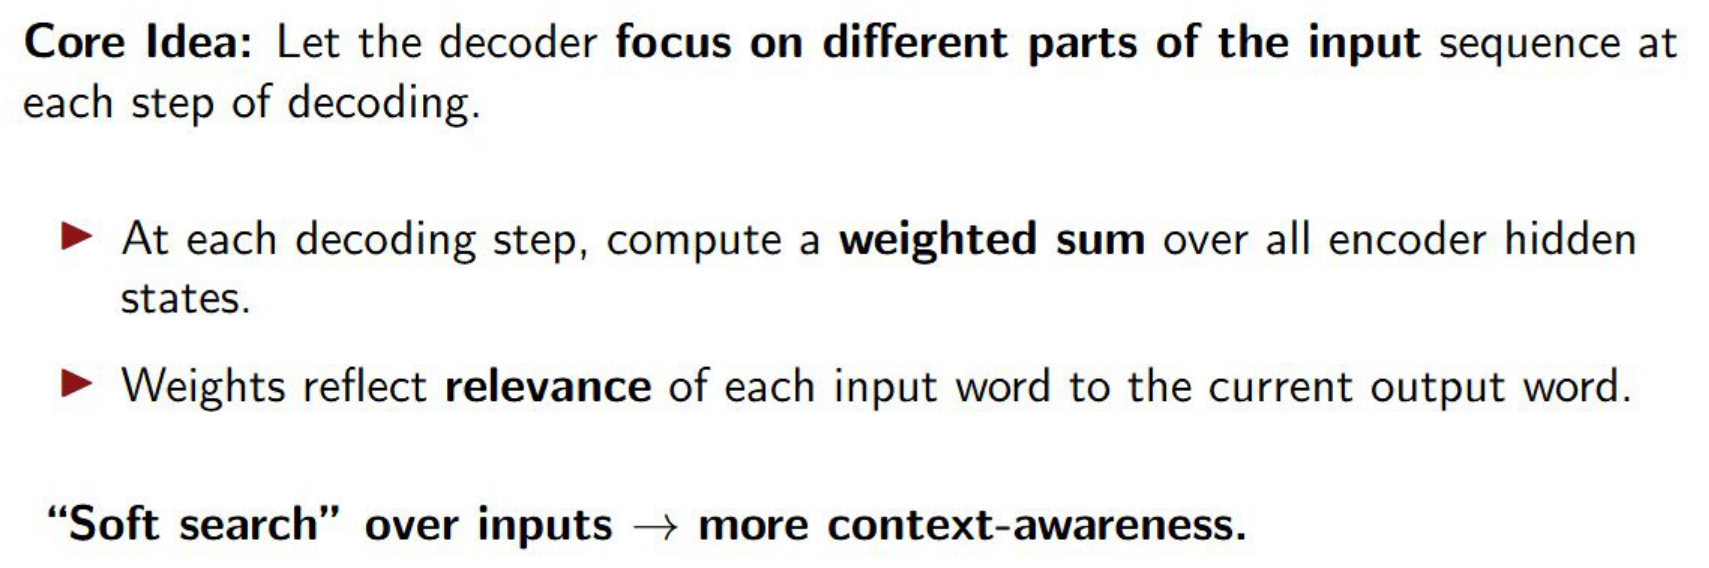
\includegraphics[width=0.4\paperwidth,height=0.4\paperheight,keepaspectratio]{assets/Lecture-4_Sequence_to_Sequence_Models_Intro_to_Attention/slide_033.png}
\end{frame}

% Slide 34
\begin{frame}{Mathematical Formulation of Attention}
  \begin{flushleft}
    \textbf{1. Alignment Score:}
    \begin{equation*}
      e_{t,s} = \text{score}(h_t^{\text{dec}}, h_s^{\text{enc}})
    \end{equation*}

    \textbf{2. Attention Weights (Softmax):}
    \begin{equation*}
      \alpha_{t, s} = \frac{\exp(e_{t, s})}{\sum_{s'} \exp(e_{t, s'})}
    \end{equation*}

    \textbf{3. Context Vector:}
    \begin{equation*}
      c_t = \sum_s \alpha_{t, s} h_s^{\text{enc}}
    \end{equation*}

    \textbf{4. Decoder Input:}
    \begin{equation*}
      y_t = \text{Decoder}(y_{t-1}, h_{t-1}^{\text{dec}}, c_t)
    \end{equation*}
  \end{flushleft}
\end{frame}

% --- PAGE 35 ---
\begin{frame}{Attention Models}
  \centering
  
\includegraphics[width=0.4\paperwidth,height=0.4\paperheight,keepaspectratio]{assets/Lecture-4_Sequence_to_Sequence_Models_Intro_to_Attention/slide_035.png}
  \begin{itemize}
      \item \textbf{Attention weights:} The weights are dynamically computed as functions of decoder state.
      \item \textbf{Expectation:} if the model is well-trained, this will automatically ``highlight'' the correct input.
      \item But how are these computed?
  \end{itemize}
\end{frame}

% --- PAGE 36 ---
\begin{frame}{Attention weights at time $t$}
  \centering
  
\includegraphics[width=0.4\paperwidth,height=0.4\paperheight,keepaspectratio]{assets/Lecture-4_Sequence_to_Sequence_Models_Intro_to_Attention/slide_036.png}  
  \begin{itemize}
      \item The ``attention'' weights $w_i(t)$ must be computed from available information at time $t$.
      \item The primary information is $s_{t-1}$ (the state at time $t-1$).
      \item Also, the input word at time $t$, but generally not used for simplicity.
  \end{itemize}
  \begin{equation*}
      c_t = \sum_{i=1}^N w_i(t) h_i
  \end{equation*}
\end{frame}

% --- PAGE 37-38 ---
\begin{frame}{Requirement on attention weights}
  \centering
  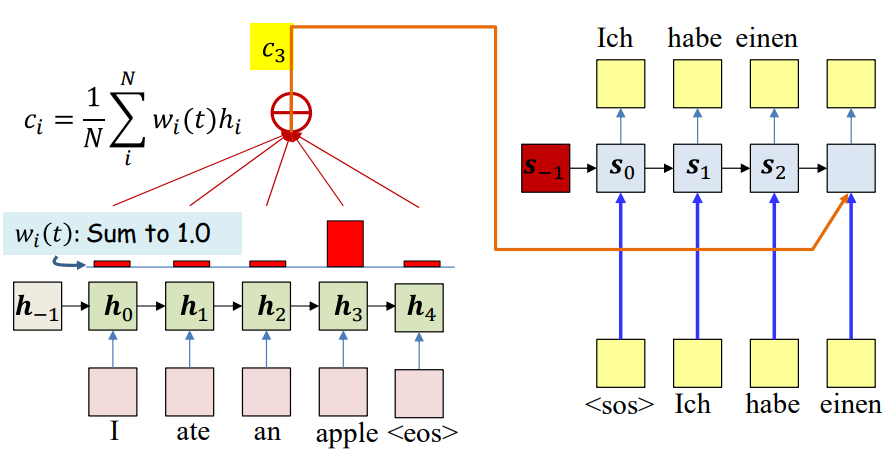
\includegraphics[width=0.4\paperwidth,height=0.4\paperheight,keepaspectratio]{assets/Lecture-4_Sequence_to_Sequence_Models_Intro_to_Attention/slide_037.png}
  \begin{itemize}
      \item The weights must be positive and sum to 1.0 (i.e., be a distribution).
      \item Ideally, they must be high for the most relevant inputs for the $i$-th output and low elsewhere.
      \item \textbf{Solution: A two step weight computation}
      \begin{itemize}
          \item First compute raw weights (which could be +ve or –ve).
          \item Then softmax them to convert them to a distribution.
      \end{itemize}
  \end{itemize}
\end{frame}

% Slide 38
\begin{frame}{Requirement on attention weights}
  \centering
  
\includegraphics[width=0.4\paperwidth,height=0.4\paperheight,keepaspectratio]{assets/Lecture-4_Sequence_to_Sequence_Models_Intro_to_Attention/slide_038.png}
  % \begin{itemize}
  %     \item The weights must be positive and sum to 1.0 (i.e., be a distribution).
  %     \item Ideally, they must be high for the most relevant inputs for the $i$-th output and low elsewhere.
  %     \item \textbf{Solution: A two step weight computation}
  %     \begin{itemize}
  %         \item First compute raw weights (which could be +ve or –ve).
  %         \item Then softmax them to convert them to a distribution.
  %     \end{itemize}
  % \end{itemize}
\end{frame}

% Slide 39
\begin{frame}{Quiz: Attention Framework}
  \begin{enumerate}
      \item The attention framework computes a different ``context'' vector at each output step?
      \item The context vector is chosen as the hidden representation of the word with the highest weight?
      \item The weight is a function of the encoder representation and the most recent decoder state?
  \end{enumerate}
\end{frame}

% Slide 40
\begin{frame}{Quiz: Answer}
  \begin{enumerate}
      \item The attention framework computes a different ``context'' vector at each output step? \textbf{True}
      \item The context vector is chosen as the hidden representation of the word with the highest weight? \textbf{False}
      \item The weight is a function of the encoder representation and the most recent decoder state? \textbf{True}
  \end{enumerate}
\end{frame}


% Slide 41
\begin{frame}{Requirement on attention weights}
  \centering
  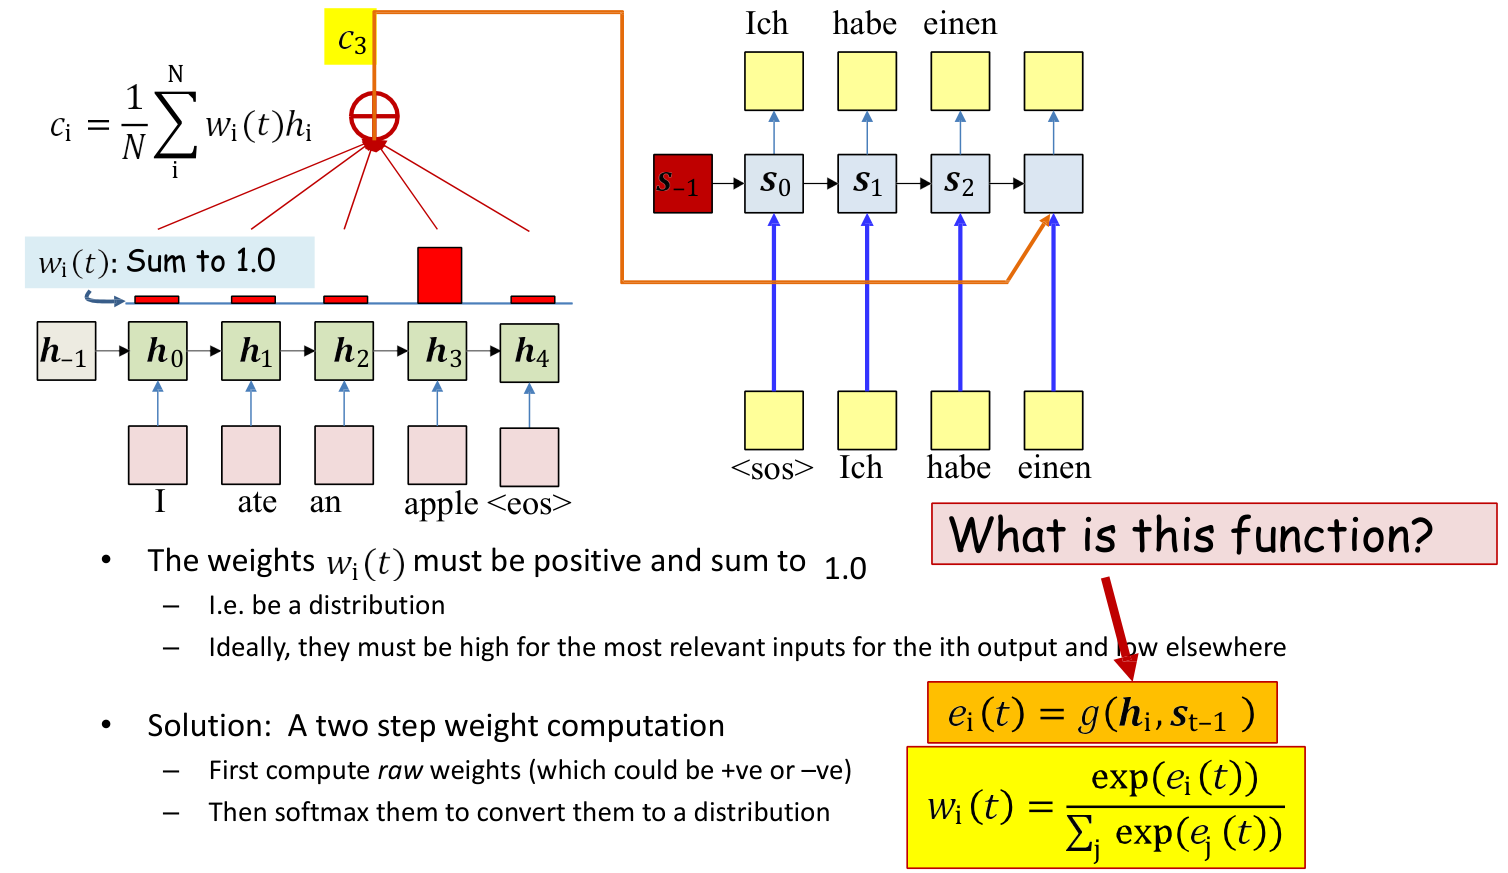
\includegraphics[width=0.4\paperwidth,height=0.4\paperheight,keepaspectratio]{assets/Lecture-4_Sequence_to_Sequence_Models_Intro_to_Attention/slide_041.png}
\end{frame}

% Slide 42
\begin{frame}{Attention weights}
  \centering
  
\includegraphics[width=0.4\paperwidth,height=0.4\paperheight,keepaspectratio]{assets/Lecture-4_Sequence_to_Sequence_Models_Intro_to_Attention/slide_042.png}
\end{frame}

\begin{frame}{Attention weights}
  \centering
  
\includegraphics[width=0.4\paperwidth,height=0.4\paperheight,keepaspectratio]{assets/Lecture-4_Sequence_to_Sequence_Models_Intro_to_Attention/slide_043.png}
\end{frame}

\begin{frame}{Converting an input: Inference}
  \centering
  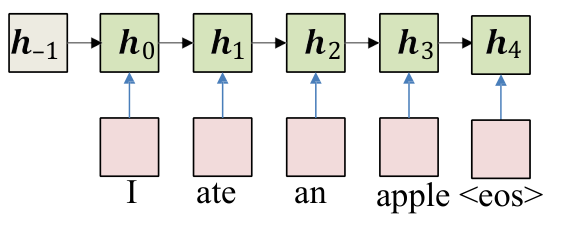
\includegraphics[width=0.4\paperwidth,height=0.4\paperheight,keepaspectratio]{assets/Lecture-4_Sequence_to_Sequence_Models_Intro_to_Attention/slide_044.png}
  Pass the input through the encoder to produce hidden representations $h_{i}$
\end{frame}

% Slide 45
\begin{frame}{Converting an input: Inference}
  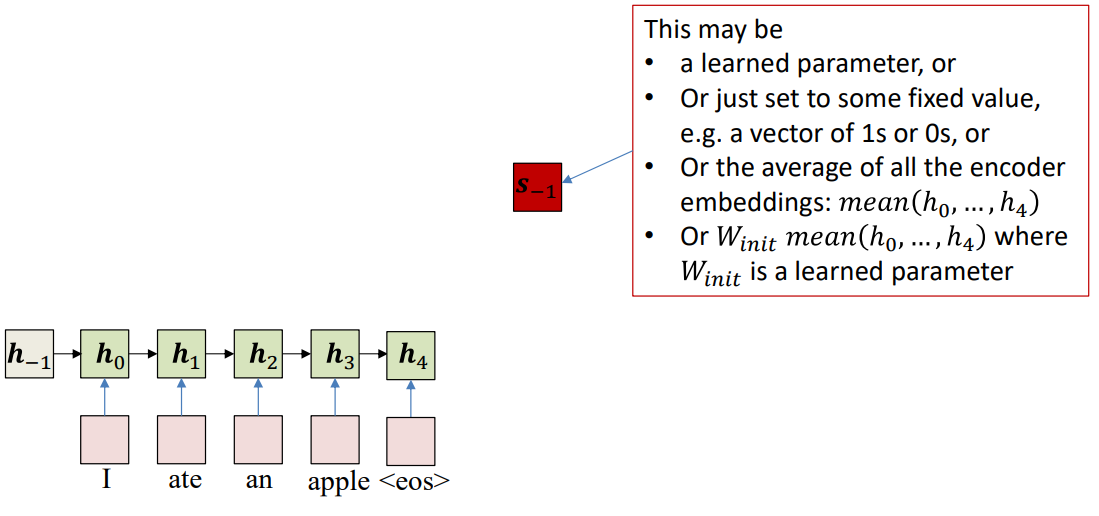
\includegraphics[width=0.4\paperwidth,height=0.4\paperheight,keepaspectratio]{assets/Lecture-4_Sequence_to_Sequence_Models_Intro_to_Attention/slide_045.png}
  \begin{itemize}
    \item[] \textbf{Pass the input through the encoder to produce hidden representations $\pmb{h_i}$}
  \end{itemize}
\end{frame}

% Slide 46
\begin{frame}{Converting an input: Inference}
  \centering
  
\includegraphics[width=0.4\paperwidth,height=0.4\paperheight,keepaspectratio]{assets/Lecture-4_Sequence_to_Sequence_Models_Intro_to_Attention/slide_046.png}
\end{frame}

% Slide 47
\begin{frame}{Converting an input: Inference}
  \centering
  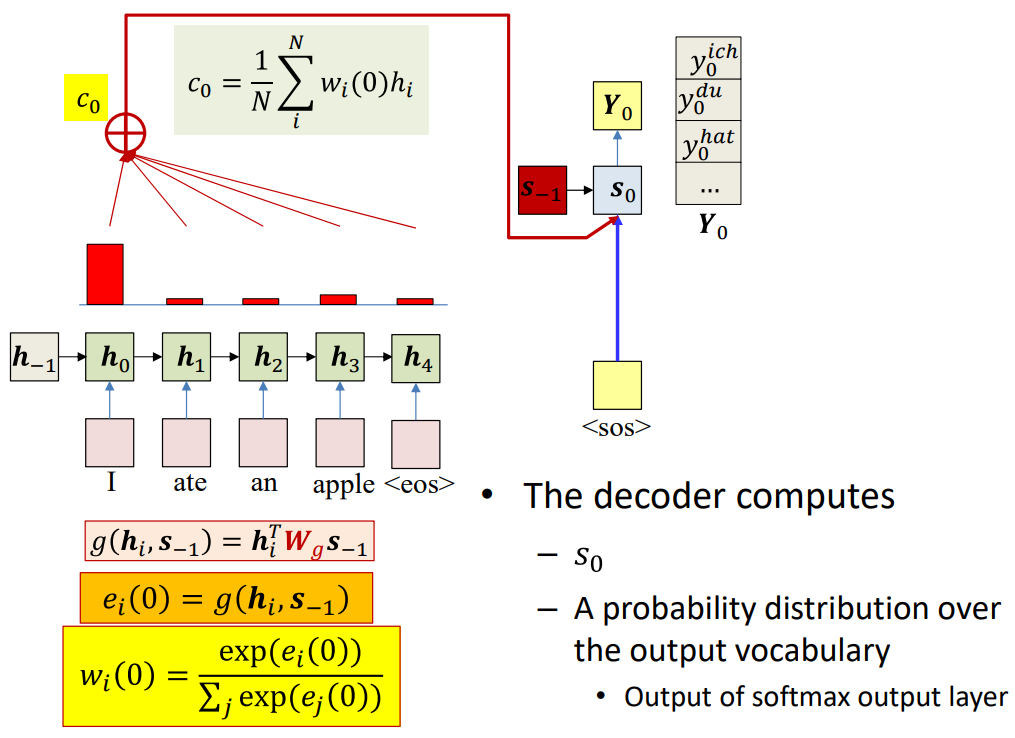
\includegraphics[width=0.4\paperwidth,height=0.4\paperheight,keepaspectratio]{assets/Lecture-4_Sequence_to_Sequence_Models_Intro_to_Attention/slide_047.png}
\end{frame}

% Slide 48
\begin{frame}{Converting an input: Inference}
  \centering
  
\includegraphics[width=0.4\paperwidth,height=0.4\paperheight,keepaspectratio]{assets/Lecture-4_Sequence_to_Sequence_Models_Intro_to_Attention/slide_048.png}
\end{frame}

% Slide 49
\begin{frame}{Converting an input: Inference}
  \centering
  
\includegraphics[width=0.4\paperwidth,height=0.4\paperheight,keepaspectratio]{assets/Lecture-4_Sequence_to_Sequence_Models_Intro_to_Attention/slide_049.png}
\end{frame}

% Slide 50
\begin{frame}{Converting an input: Inference}
  \centering
  
\includegraphics[width=0.4\paperwidth,height=0.4\paperheight,keepaspectratio]{assets/Lecture-4_Sequence_to_Sequence_Models_Intro_to_Attention/slide_050.png}
\end{frame}

% Slide 51
\begin{frame}{Converting an input: Inference}
  \centering
  
\includegraphics[width=0.4\paperwidth,height=0.4\paperheight,keepaspectratio]{assets/Lecture-4_Sequence_to_Sequence_Models_Intro_to_Attention/slide_051.png}
\end{frame}


% Slide 52
\begin{frame}{Converting an input: Inference}
  \centering
  
\includegraphics[width=0.4\paperwidth,height=0.4\paperheight,keepaspectratio]{assets/Lecture-4_Sequence_to_Sequence_Models_Intro_to_Attention/slide_052.png}
\end{frame}

% Slide 53
% \begin{frame}{Converting an input: Inference}
%   \centering
%   
\includegraphics[width=0.4\paperwidth,height=0.4\paperheight,keepaspectratio]{assets/Lecture-4_Sequence_to_Sequence_Models_Intro_to_Attention/slide_053.png}
% \end{frame}

% Slide 54
\begin{frame}{Converting an input: Inference}
  \centering
  
\includegraphics[width=0.4\paperwidth,height=0.4\paperheight,keepaspectratio]{assets/Lecture-4_Sequence_to_Sequence_Models_Intro_to_Attention/slide_054.png}
\end{frame}

% Slide 55
\begin{frame}{Attention-based Decoding}
  \centering
  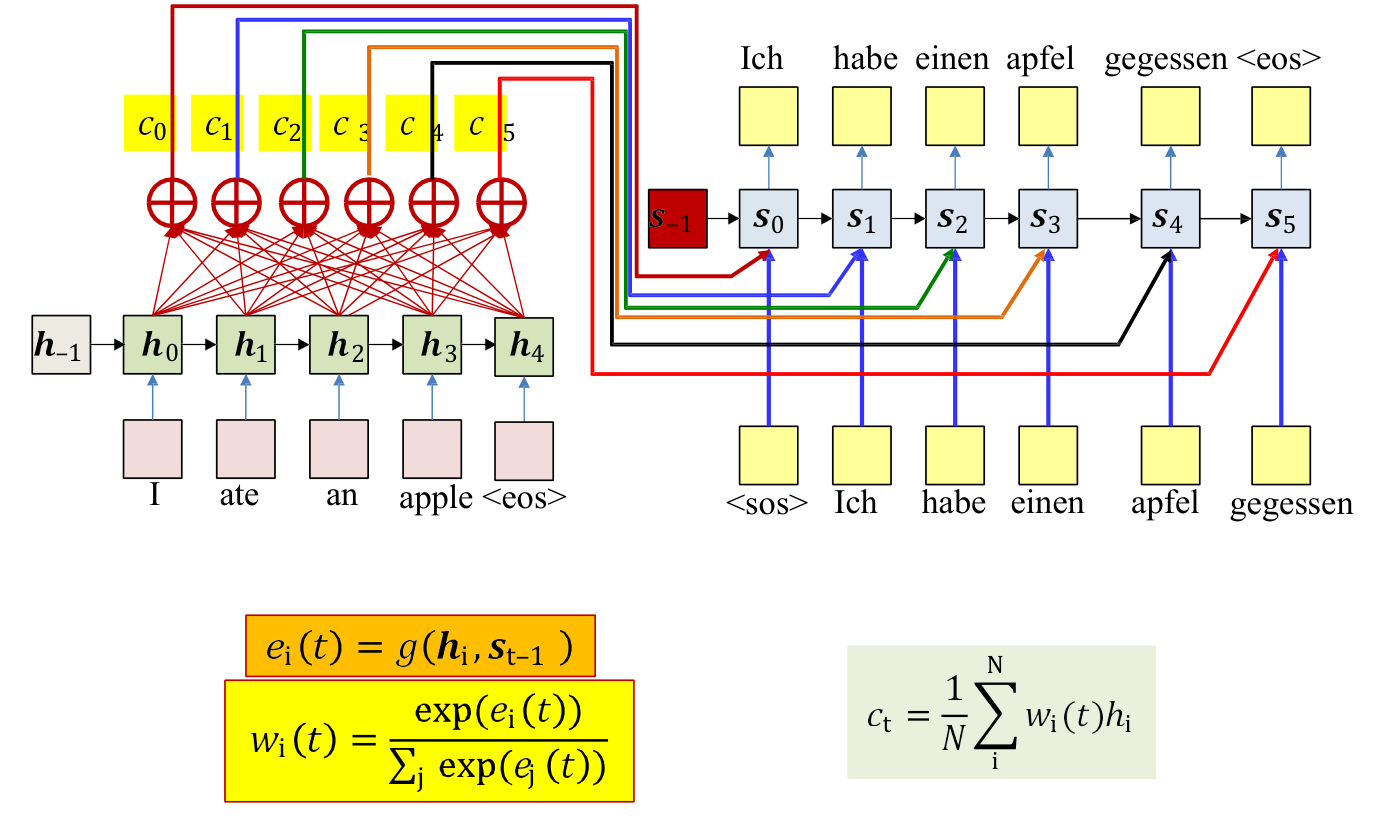
\includegraphics[width=0.4\paperwidth,height=0.4\paperheight,keepaspectratio]{assets/Lecture-4_Sequence_to_Sequence_Models_Intro_to_Attention/slide_055.png}
\end{frame}

% Slide 56
\begin{frame}{Recap: Sequence to Sequence Models}
  \centering
  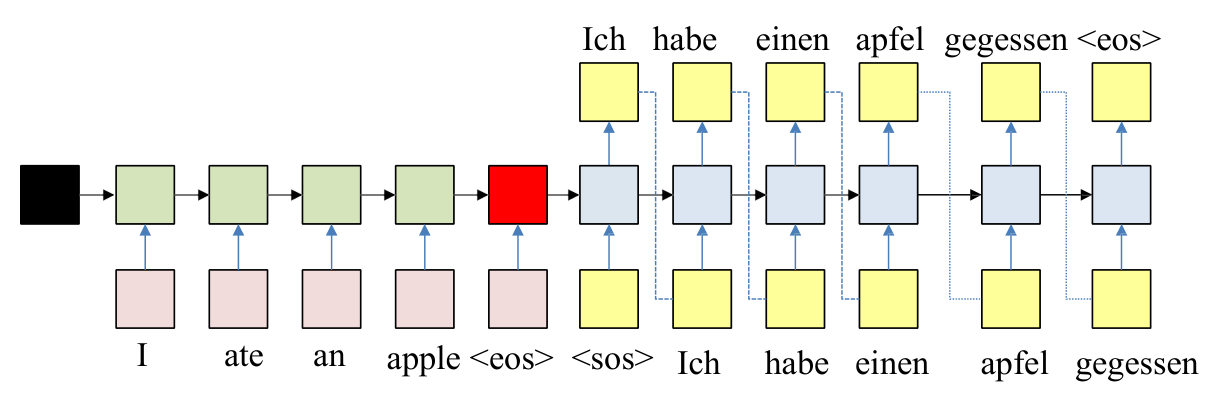
\includegraphics[width=0.4\paperwidth,height=0.4\paperheight,keepaspectratio]{assets/Lecture-4_Sequence_to_Sequence_Models_Intro_to_Attention/slide_056.png}
\begin{itemize}
  \item The input sequence feeds into a recurrent structure
  \item The input sequence is terminated by an explicit \textless eos\textgreater{} symbol
    \begin{itemize}
      \item \textcolor{red}{The hidden activation at the \textless eos\textgreater{} ``stores'' all information about the sentence}
    \end{itemize}
  \item Subsequently a second RNN uses the hidden activation as initial state to produce a sequence of outputs
\end{itemize}
\end{frame}

% Slide 57
\begin{frame}{Recap: Attention Models}
  \centering
  
\includegraphics[width=0.4\paperwidth,height=0.4\paperheight,keepaspectratio]{assets/Lecture-4_Sequence_to_Sequence_Models_Intro_to_Attention/slide_057.png}
\begin{itemize}
  \item Encoder recurrently produces hidden representations of input word sequence
  \item Decoder recurrently generates output word sequence
    \begin{itemize}
      \item For each output word the decoder uses a weighted average of the hidden input representations as input ``context'', along with the recurrent hidden state and the previous output word
    \end{itemize}
\end{itemize}
\end{frame}

% Slide 58
\begin{frame}{Recap: Attention Models}
  \centering
  
\includegraphics[width=0.4\paperwidth,height=0.4\paperheight,keepaspectratio]{assets/Lecture-4_Sequence_to_Sequence_Models_Intro_to_Attention/slide_058.png}
\begin{itemize}
  \item \textbf{Problem:} Because of the recurrence, the hidden representation for any word is also influenced by \emph{all} preceding words
    \begin{itemize}
      \item The decoder is actually paying attention to the sequence, and not just the word
    \end{itemize}
\end{itemize}
\end{frame}
